%====================================================================================================
% ?????
%====================================================================================================
% TCC
%----------------------------------------------------------------------------------------------------
% Autor				: Jasane Schio
% Orientador		: Gedson Faria
% Co-Orientador		: Angelo Darcy
% Instituição 		: UFMS - Universidade Federal do Mato Grosso do Sul
% Departamento		: CPCX - Sistema de Informação
%----------------------------------------------------------------------------------------------------
% Data de criação	: 01 de Outubro de 2015
%====================================================================================================
% NO FUTURO
\chapter{Introdução} \label{Cap:Introducao}
\section{Considerações Iniciais}
Em 1997 foi estabelecida a Federation of International Robot-soccer Association (FIRA), com o intuito de promover o desenvolvimento nas áreas de multi-agentes autonomos e cooperação entre robôs, bem como pesquisas e estudos relacionados a mecatrônica, processamento de imagens e robótica\cite{FiraHistory,FiraOverview}. O Futebol de Robôs tem sido  uma das principais áreas de foco por ser um domínio complexo, exigindo autonomia do sistema e solução de problemas em tempo real\cite{Costa:2000,Faria2006}. 

Nos jogos de futebol, o técnico passa as informações pessoalmente para seus jogadores em campo, porem isso não é possível no futebol de robôs, já que neste ambiente tais informações precisam ser passadas via comunicação de dados.%, no qual cada um dos robôs se difere do outro por obter um identificador único. 
Os robôs são diferenciados computacionalmente por um identificador único (e.g. endereço MAC) e em sua carcaça por marcadores com duas cores, uma cor designando o time a qual o robô pertence e outra que o identifica de maneira única dentro de sua equipe. O software de estratégia de cada equipe deve detectar os marcadores de cor utilizando técnicas de visão computacional e decidir a partir da posição dos robôs em campo qual atitude será realizada.

Para identificar cada uma das cores devem considerados alguns fatores como: a iluminação local, a tonalidade de cor dos marcadores, a posição dos refletores e sombras sobre o campo, portanto, é necessário que se faça o processo chamado de calibração. A calibração de cores ocorre para designar o intervalo de valores que corresponde a cada cor naquele determinado momento. Intervalos de cores podem ser pré definidos, no entanto, de acordo a mudança de qualquer um dos fatores já citados, uma nova calibração se faz necessária.



\section{Trabalhos Correlatos}
Para o tema específico deste trabalho, calibração de intervalo de cores para times de futebol de robôs da categoria IEEE Very Small Size Soccer, não foram encontrados trabalhos relacionados, porém foram encontrados Team Discription Papers e descrições de sistemas usados pelos times\cite{Penharbel:2004}\cite{Rosa:2015}\cite{VSSVision}\cite{PenharbelTime}.

\subsection{Calibra}
O Centro Universitário da FEI propôs o sistema denominado CALIBRA, desenvolvido para sistemas Linux e com {\it Graphical User Interface}. O sistema de calibração possui um módulo chamado de {\it MainWindow} que disponibiliza a configuração de brilho, cor e contraste da imagem adquirida pela câmera, e grava estas configurações em um arquivo que é utlizado no momento de definir os intervalos no espaço de cores HSI para cada uma das cores dos marcadores de identificação dos robôs\cite{Penharbel:2004,PenharbelTime}. Deve-se ressaltar que a descriçao do sistema CABLIBRA n~ao contempla os detalhes de implementaç~ao da calibração das cores.
\begin{figure}[H]
	\centering
	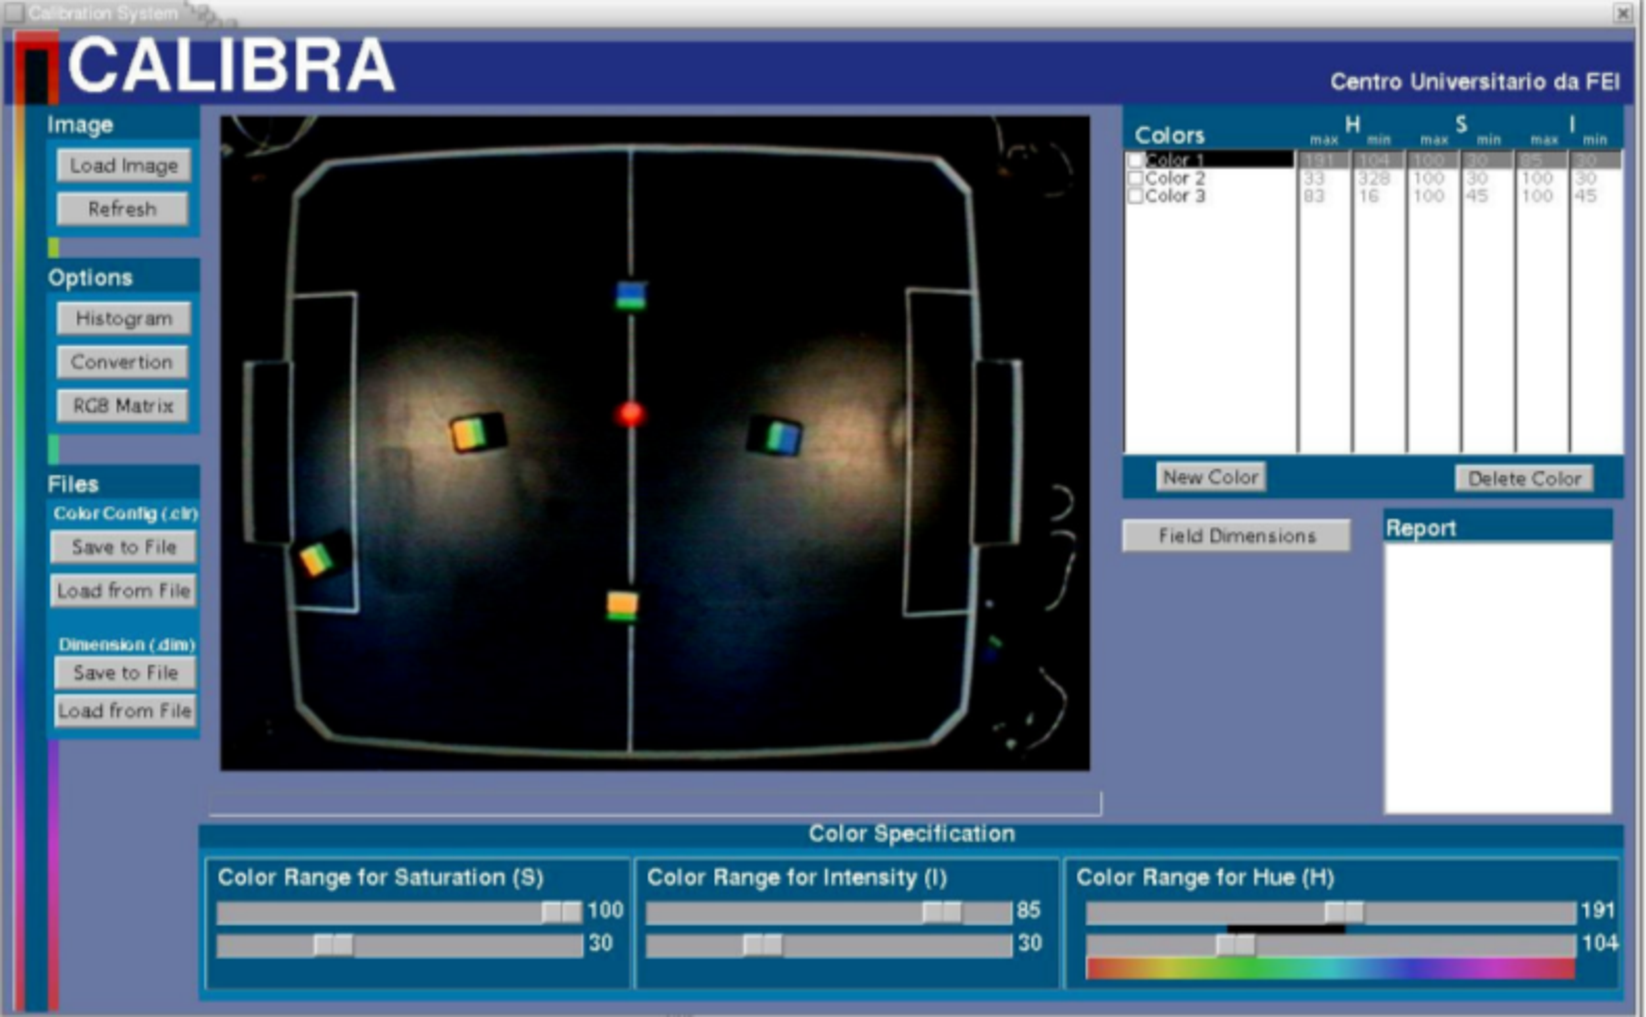
\includegraphics[width=0.6\textwidth]{calibra.pdf}
	\caption{Sistema Calibra, FEI\cite{Penharbel:2004}}
	\label{Calibra}
\end{figure}

\subsection{VSS-Vision}

O VVS-Vision é um sistema completo de controle da equipe de futebol de robôs da categoria {\it IEEE Very Small Size Soccer}(VSSS) do Laboratório de Sistemas Inteligentes e Robótica (SIRLab) da Faeterj/Petrópolis \cite{Rosa:2015}. Este sistema de contempla a calibaração de cores e foi utilizado durante a competição XXXXY (LARC) do ano de 2014.

\begin{figure}[H]
	\centering
	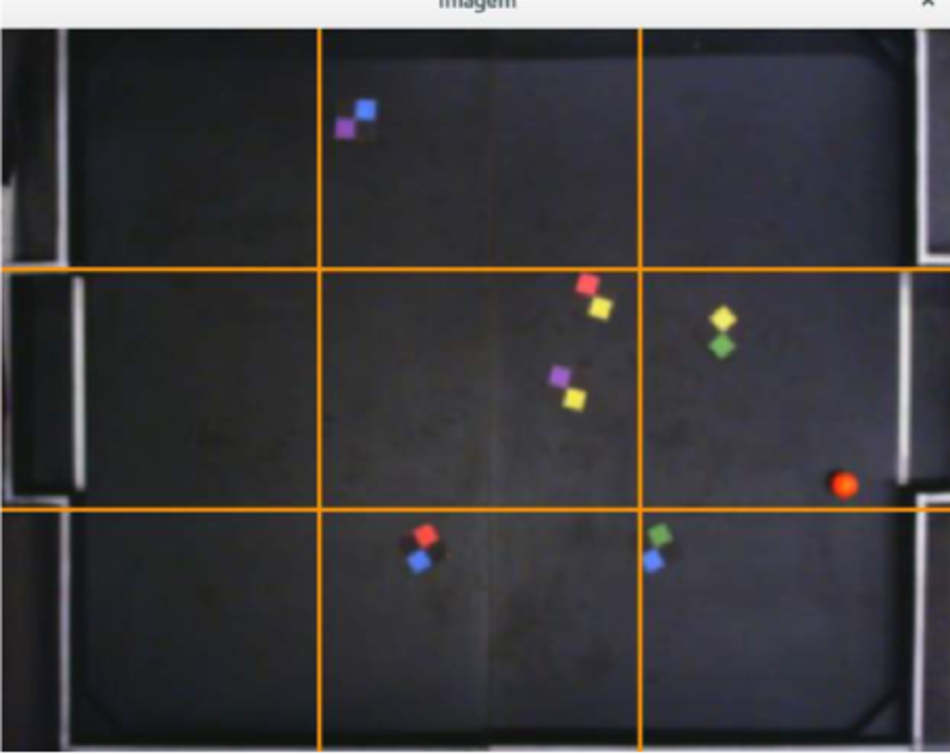
\includegraphics[width=0.4\textwidth]{vssvision.pdf} 	
	\caption{Sistema de calibracao, SIRLab\cite{Rosa:2015}}
	\label{SIRLabCalibracao}
\end{figure}
Rosa menciona que a calibração de cores e feita calibrando obrigatoriamente laranja, amarelo e azul, e então as outras cores referentes aos jogadores em campo. Como visto na Figura \ref{SIRLabCalibracao} a imagem da c\^amera é dividida em nove cantos, e para calibrar a cor o usuário deve clicar em cima da cor que gostaria de ser calibrada, assim salvando um intervalo de cor tratado como RGB máximo e o mínimo daquela cor , a medida
que vão havendo os cliques o sistema verifica para cada atributo se ele é maior que o atributo
máximo salvo ou menor que mínimo salvo, caso seja, o mesmo assume o lugar de menor ou
maior e esse processo deve ser feito em cada um dos nove cantos da imagem\cite{Rosa:2015}. 
%Os valores HSV encontrados s\~ao ajustados manualmente com a ajuda de sliders, como visto na Figura \ref{SIRLabCalibracaoHSV}. Este processo de calibração pode demorar entre cinco e dez minutos.
O desenvolvimento do sistema utiliza para processamento de imagens a biblioteca OpenCV e para telas interativas a biblioteca  ImGui.

%\begin{figure}[!h]
%	\centering
%	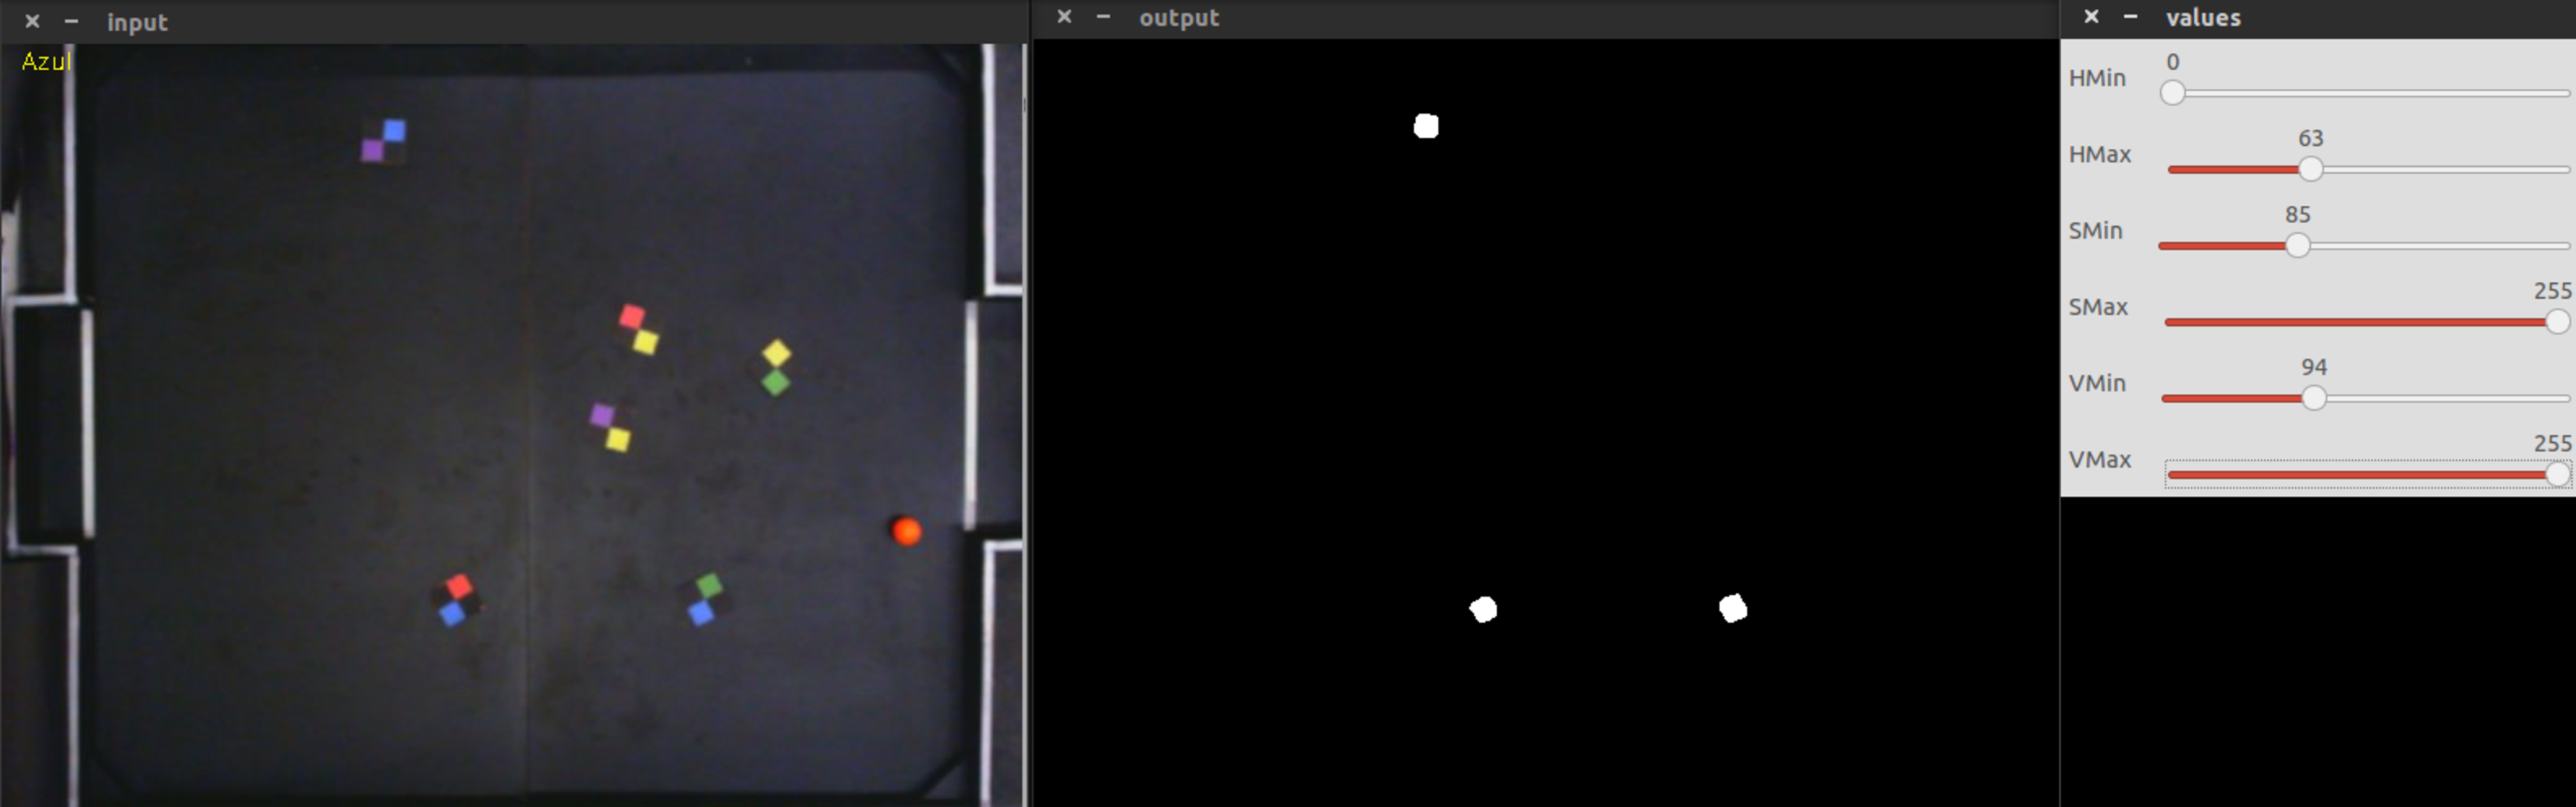
\includegraphics[width=0.8\textwidth]{calibration.pdf} 	
%	\caption{Sistema de calibracao, SIRLab\cite{VSSVision}}
%	\label{SIRLabCalibracaoHSV}
%\end{figure}

O atual sistema de visão computacional do SIRLab passou por algumas mudanças desde 2015 e conta com uma inteface e metodo de calibração diferentes\cite{VSSVision}. Como disponível no repositorio online do Laboratorio, o atual sistema de calibração de cores utiliza o espaço de cores HSV, no lugar do RGB\cite{Rosa:2015}. A antiga interface do sistema, feita inicialmente em ImGui deu lugar a nova, desenvolvida em Qt, como mostra a Figura \ref{SIRLabNova}.

O método de calibração de cores também foi modificado, o sistema possibilita a calibragem de 8 cores, Laranja, Amarelo, Azul, Vermelho, Verde, Rosa, Roxo, Marrom\cite{VSSVision}. Após o usuário escolher uma cor para calibrar o mesmo deve encontrar um intervalo de cor, no espaço de cores HSV, que represente-a. Ao clicar na tela com o botão direito o sistema da um zoom na área para ajuste fino. A Figura \ref{SIRLabNovaCalibracao} demonstra o novo método de calibração.
\begin{figure}[H]
\begin{minipage}[H]{0.45\linewidth}
\hspace{0.5cm}
\centering
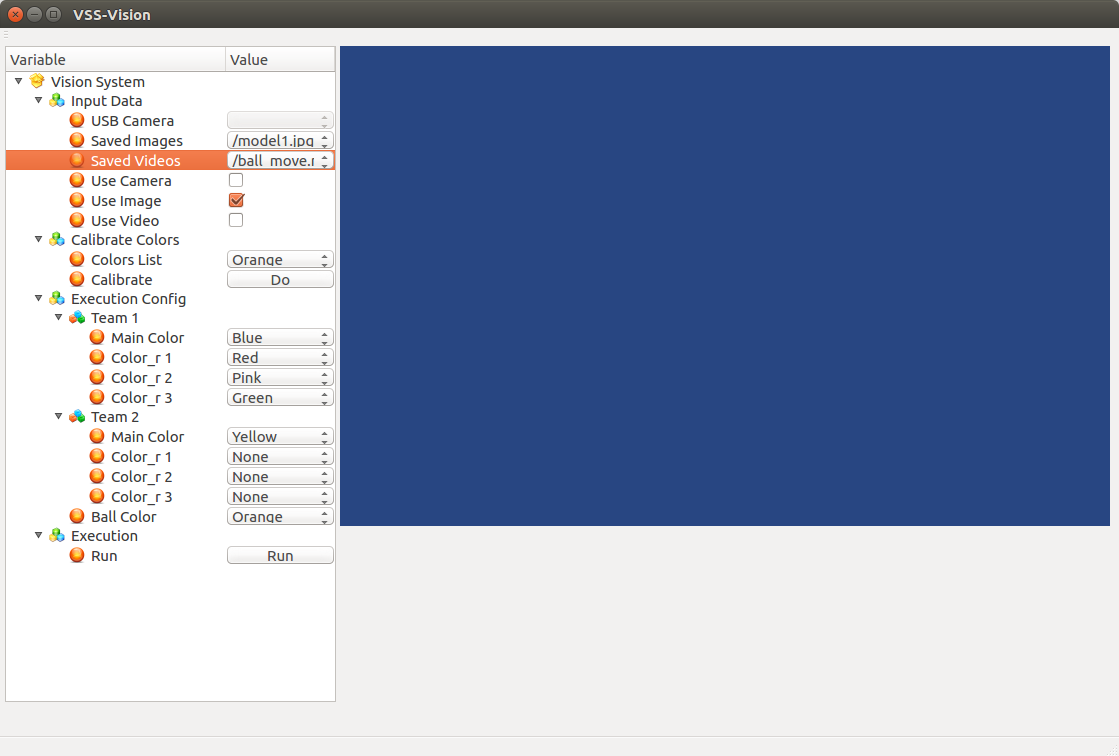
\includegraphics[width=\textwidth]{vsssnovonormal.png}
\caption{Nova interface do sistema de calibração da SIRLab\cite{VSSVision}}
\label{SIRLabNova}
\end{minipage}
\hspace{0.5cm}
\begin{minipage}[H]{0.40\linewidth}
\centering
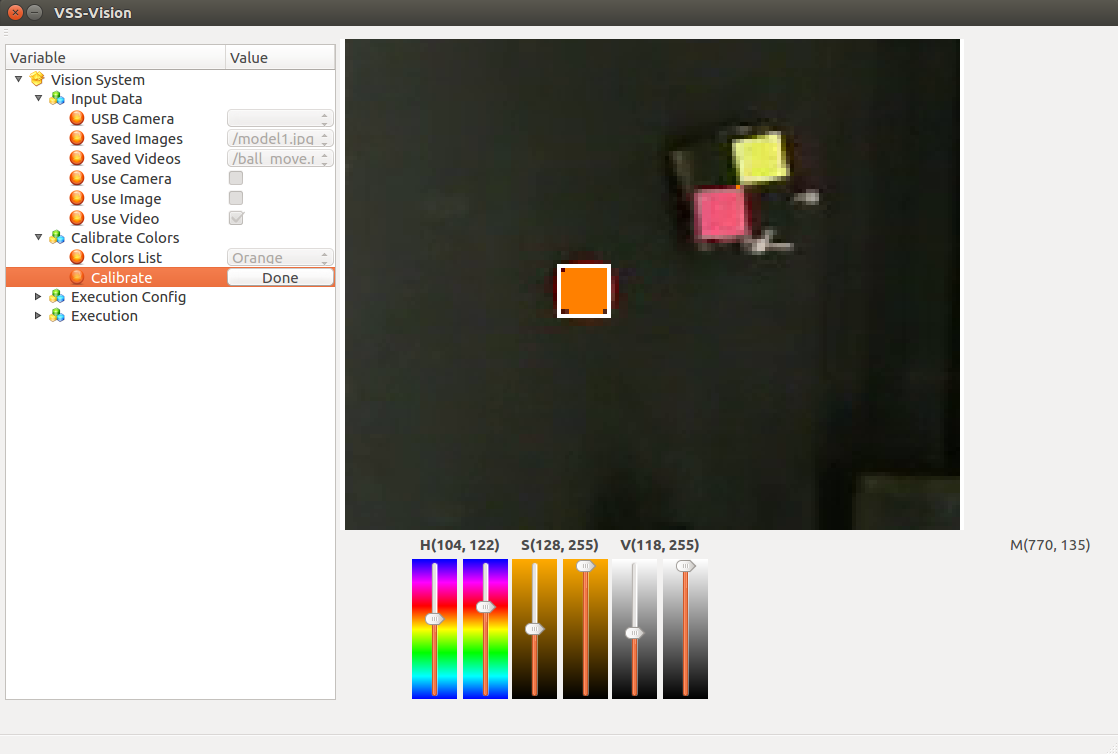
\includegraphics[width=\textwidth]{vsssnovo.png}
\caption{Atual Sistema de calibração da SIRLab\cite{VSSVision}}
\label{SIRLabNovaCalibracao}
\end{minipage}
\end{figure}	

\section{Motivação e Justificativa}
Em 2015 surgiu a equipe Cedro, equipe de futebol de robôs categoria IEEE Very Small Size Soccer da UFMS Campus Coxim. Já em seu primeiro ano a equipe participou da Competição Latino Americana de Robótica, competição cuja qual tive a oportunidade de participar como membro da equipe. Como minha primeira vez em um evento deste âmbito, fiz algumas observações sobre as equipes e as partidas, a principal foi quanto a calibração de cores. De forma informal, todo jogo possue um \emph{aquecimento} de 20 minutos, tempo esse que a maioria das equipes utilizada deste tempo para fazer a calibração de cores. Na equipes que observei, o processo de calibração foi feita de forma manual com uma interface muito semelhante ao deselvolvido por Kyle Hounslow\cite{YouTube}. Em algumas equipes, inclusive foi desenvolvido um novo modelo de cores, como é o caso da POTI/UFRN\cite{Martins:2007}.

Foi estudado o problema da calibração de cores para competição de futebol de robôs categoria IEEE VSSS, na qual a calibração de cada uma das cores em campo acaba se tornando um processo exaustivo por ter de ser feito um a um, cerca de 5 minutos para cada cor. Geralmente o tempo de preparo inicial antes de cada jogo é de 20 minutos, tempo que acaba sendo gasto praticamente inteiro no processo de calibração. Se o processo de calibração fosse automatizado, e assim reduzido, haveria mais tempo para ser usado em melhorias técnicas, hardware dos robôs com problemas, melhorias na estratégia de jogo ou resolvendo problema de comunicação. Devido ao problema citado percebeu-se o beneficio de se desenvolver um sistema autônomo de registro do valores HSV que faça a definição de intervalos de cores baseando-se nos objetos em campo, os identificando de forma automática, assim diminuindo o alto tempo gasto na calibração de cores 
\section{Objetivos}
Neste trabalho tem-se por objetivo principal automatizar o sistema de identificação de objetos 
coloridos em imagens provenientes de uma câmera em imagens de tempo real, fazendo a calibração dos valores HSV identificando seus limites mínimos e máximos.  
Para desenvolver um sistema que supra essas necessidades, foram propostos os seguintes objetivos específicos:

\begin{itemize}
	
	\item Estudar e implementar a detecção automática dos objetos em campo; 
	\item Estudo de cores para identificação de intervalos de cores dentro da biblioteca OpenCV;
	\item Categorização das cores dos objetos identificados dentro dos intervalos estudados;
	\item Testar o sistema proposto para identificação de cores.
	
	
\end{itemize}

\newpage

\section{Organização da Trabalho} \label{Sec:Organizacao}

Este trabalho está divido em cinco capítulos. No segundo capítulo encontra-se a fundamentação teórica, contento informações sobre processamento de imagens referente à detecção de objetos e cores e uma breve descrição sobre o futebol de robôs. No terceiro capítulo encontra-se todo o desenvolvimento do projeto, suas classes, a descrição das tecnologias utilizadas no projeto, e a descrição do processo de calibração. No quarto capítulo são apresentados os testes e discutidos os resultados obtidos. No quinto capítulo são feitas as conclusões do trabalho, bem como expostas melhorias que possam vir a ser implementadas em trabalhos futuros.

\section{Considerações Finais}
